\section*{Apêndice B -- Representações bidimensionais dos ligantes utilizados}
\refstepcounter{apendice}
\phantomsection
\label{ap:estruturas_ligantes}

Os painéis apresentam os 34 registros do inventário atual. As estruturas foram desenhadas no RDKit 2025.09.4 a partir dos SMILES registrados nos PDBQT de 1H1B, conferidos com os arquivos correspondentes de 2PE4. Cada representação preserva a conectividade e a estereoquímica registradas, sem representar a pose tridimensional ou suas cargas parciais.

\begin{figure}[H]
\centering
\caption[Ligantes comerciais e de referência (1/2)]{Representações bidimensionais dos ligantes comerciais e de referência: painel 1 de 2, com os nove primeiros registros do inventário.}
\label{fig:estruturas_comerciais_01}
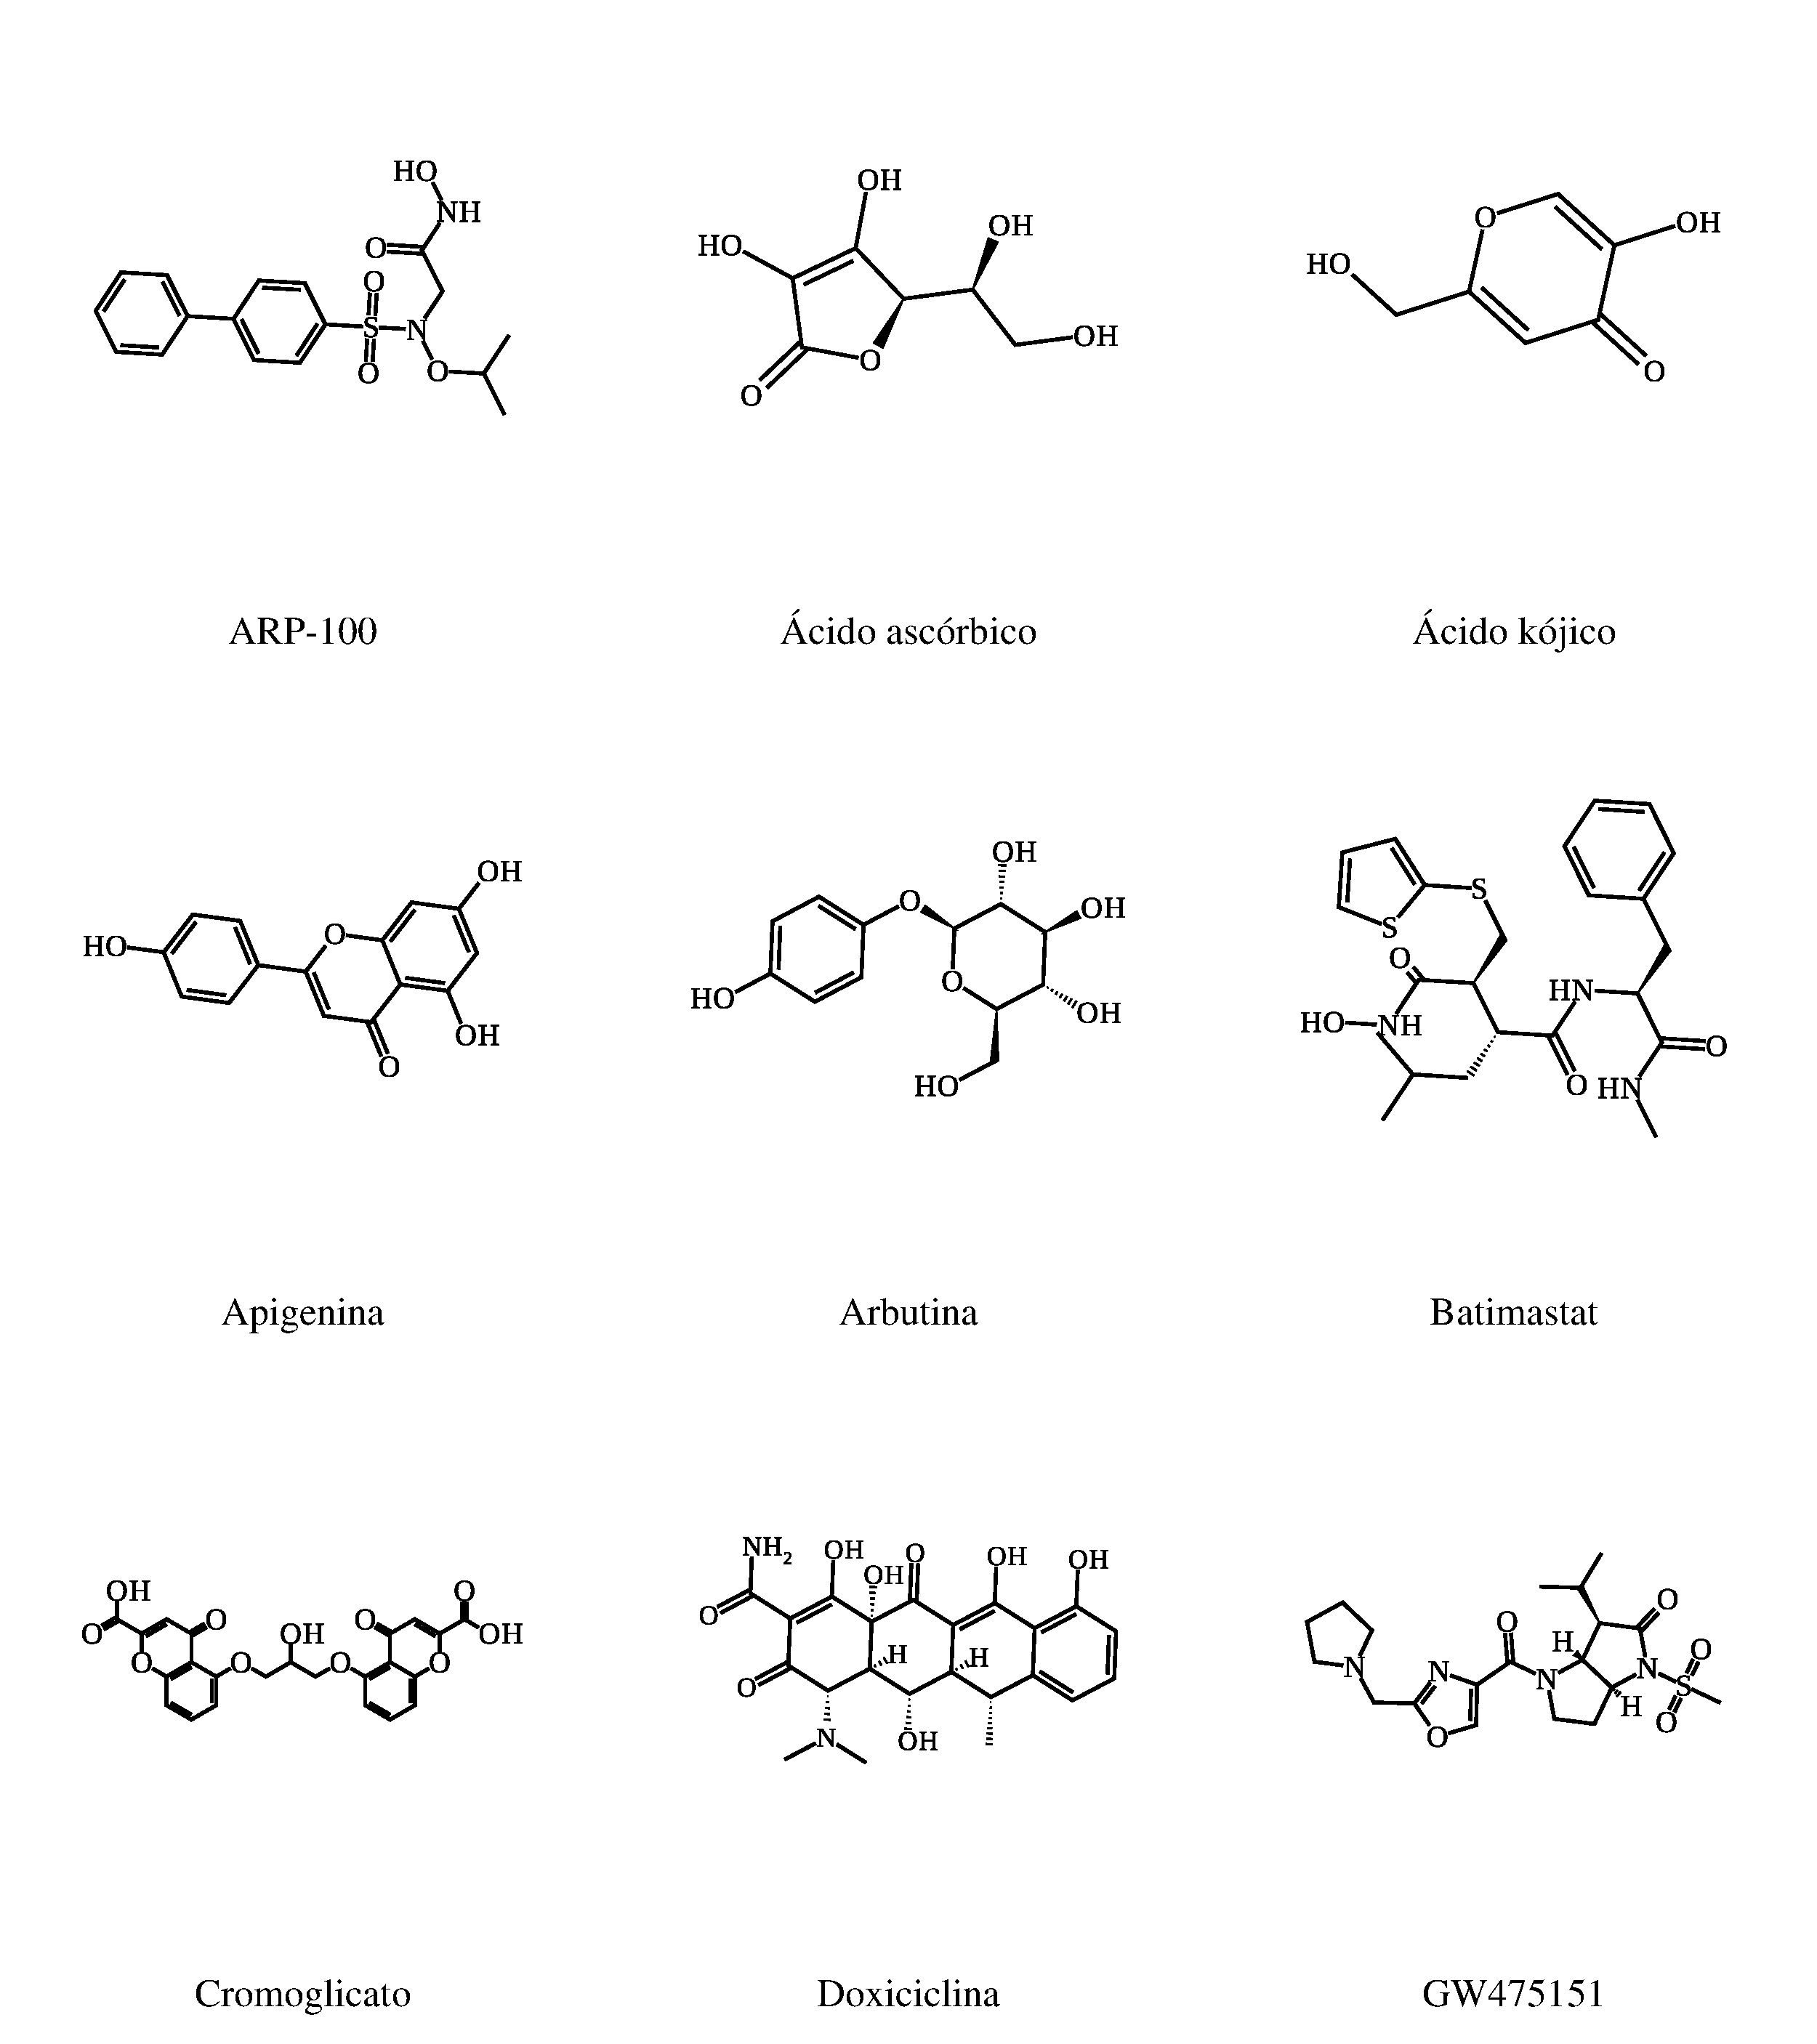
\includegraphics[width=\linewidth,height=17.4cm,keepaspectratio]{image/estruturas_ligantes_integracao/comerciais_01.pdf}
\end{figure}

\clearpage
\begin{figure}[H]
\centering
\caption[Ligantes comerciais e de referência (2/2)]{Representações bidimensionais dos ligantes comerciais e de referência: painel 2 de 2, com os oito registros restantes. L2U ocupa duas colunas para facilitar a leitura.}
\label{fig:estruturas_comerciais_02}
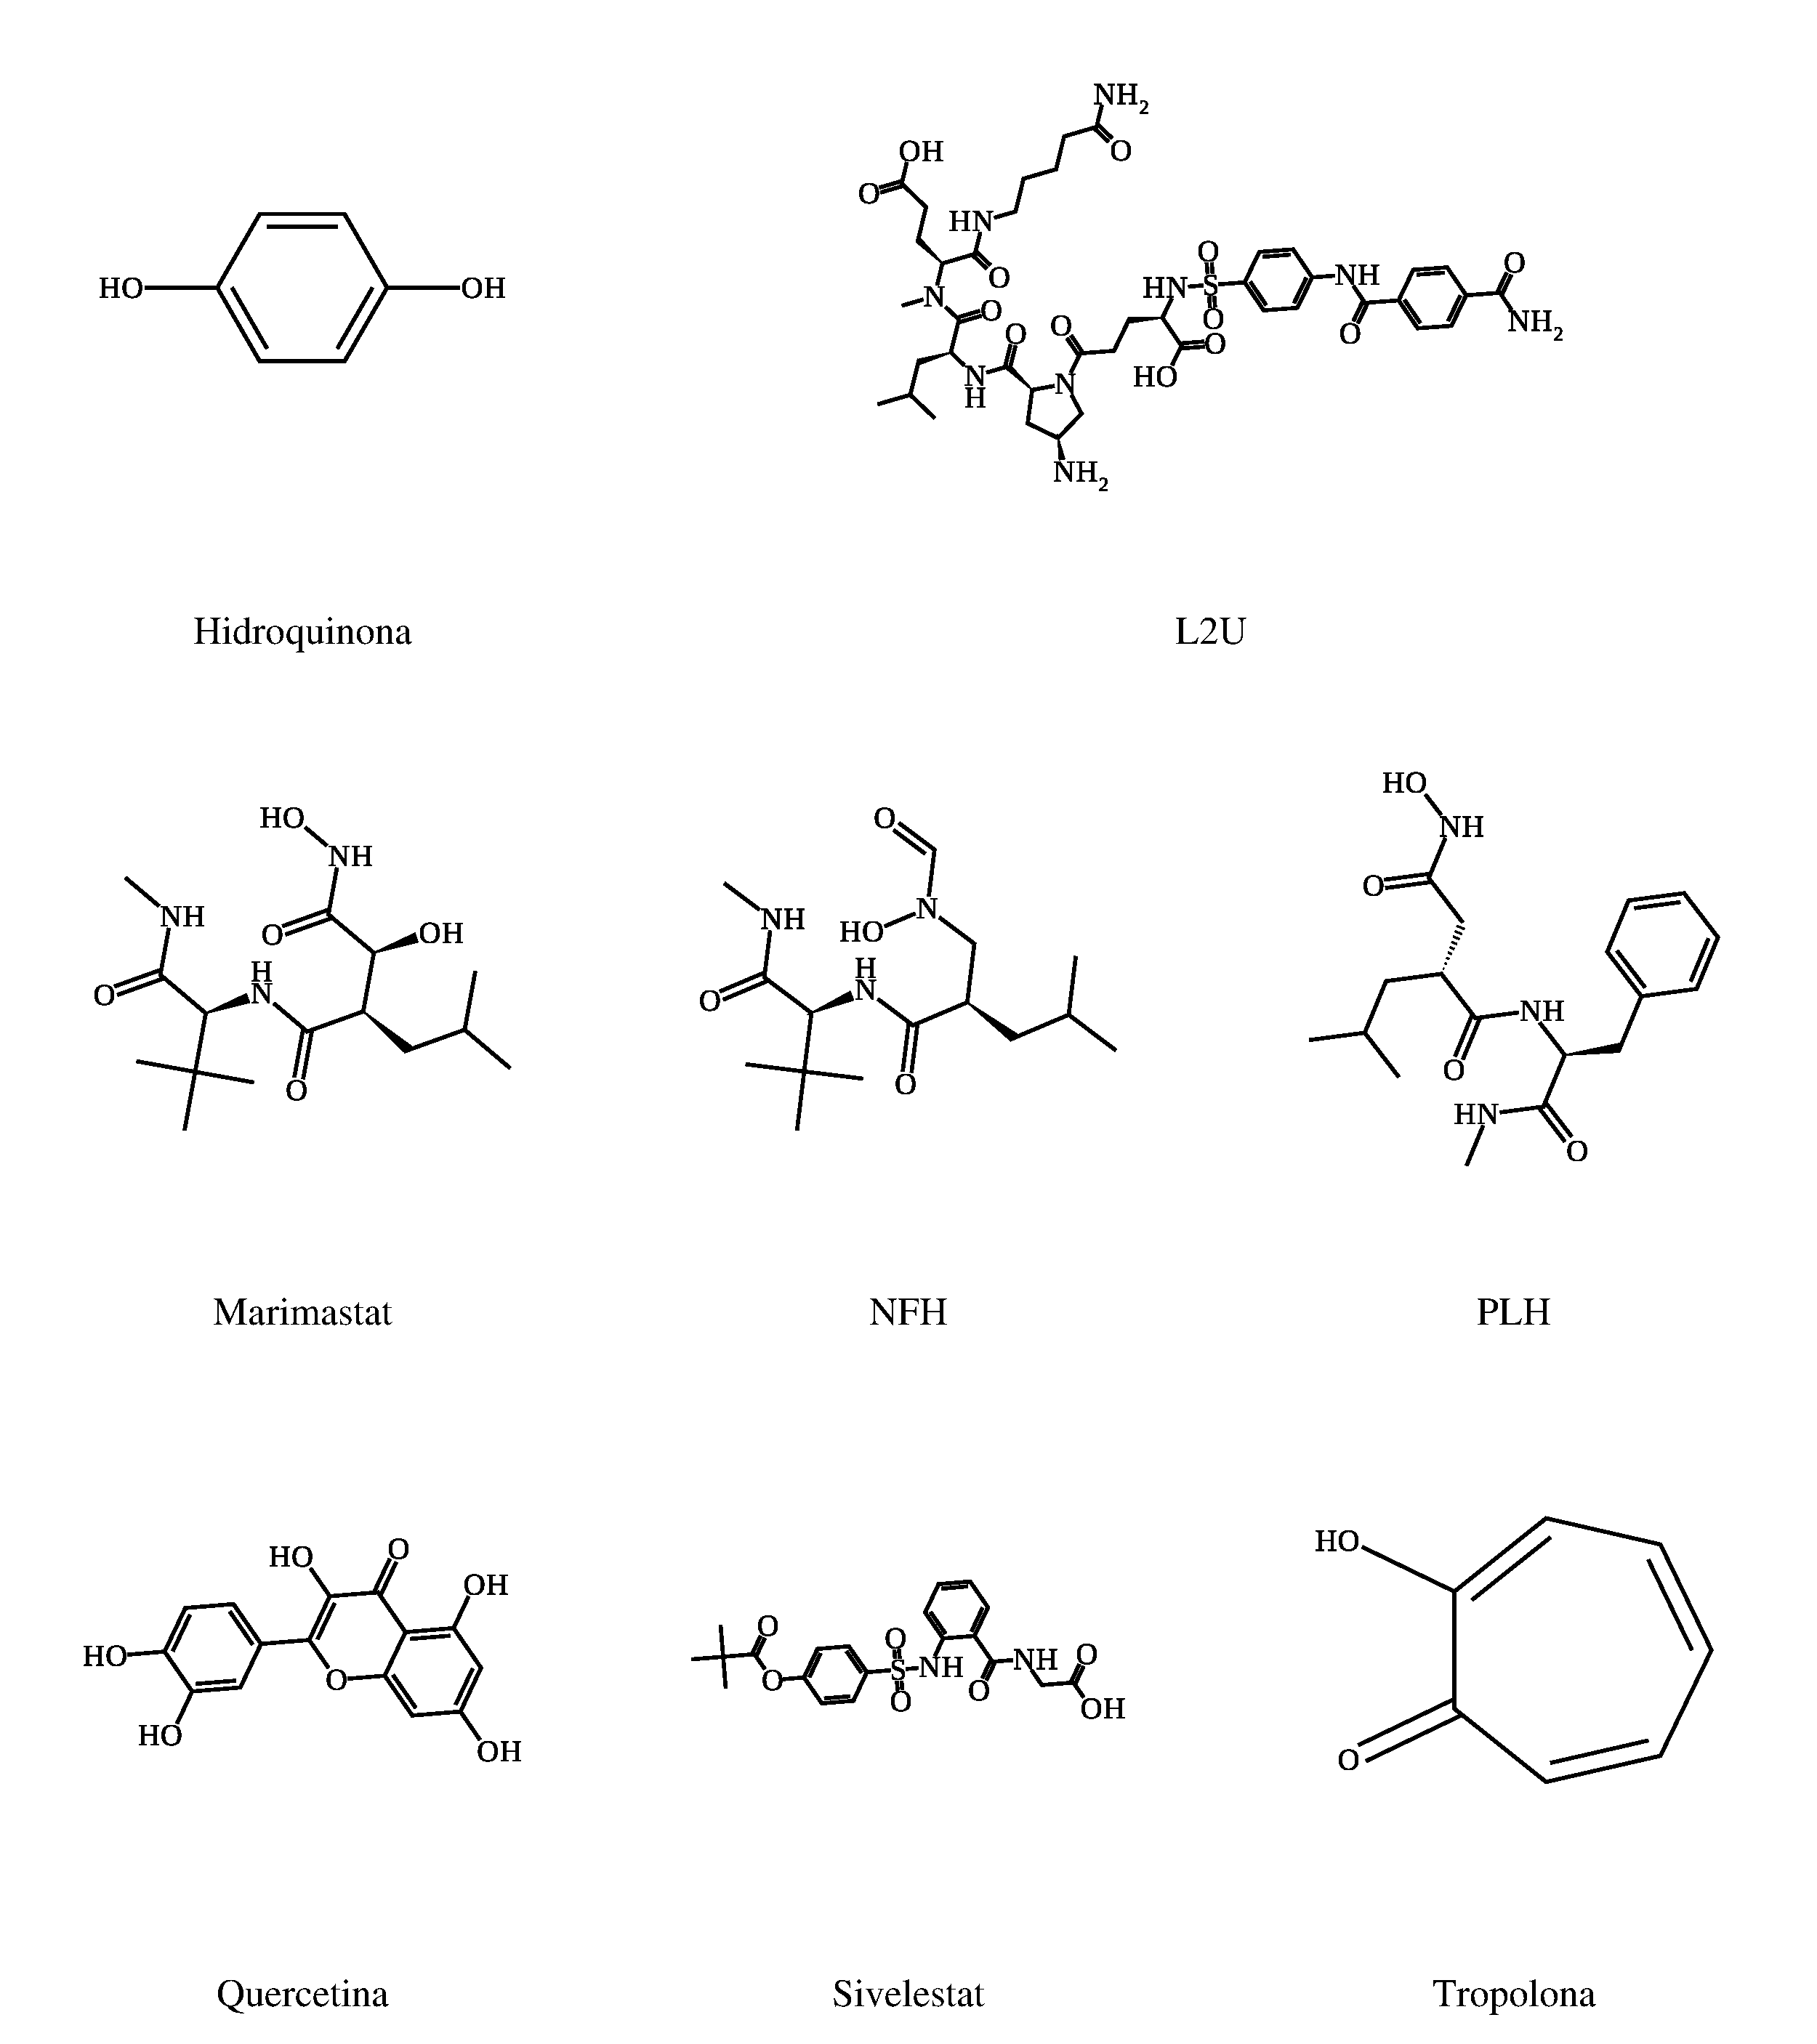
\includegraphics[width=\linewidth,height=18cm,keepaspectratio]{image/estruturas_ligantes_integracao/comerciais_02.pdf}
\end{figure}

\clearpage
\begin{figure}[H]
\centering
\caption[Compostos para prospecção (1/2)]{Representações bidimensionais dos compostos selecionados para prospecção: painel 1 de 2, com os nove primeiros registros do inventário.}
\label{fig:estruturas_tetra_01}
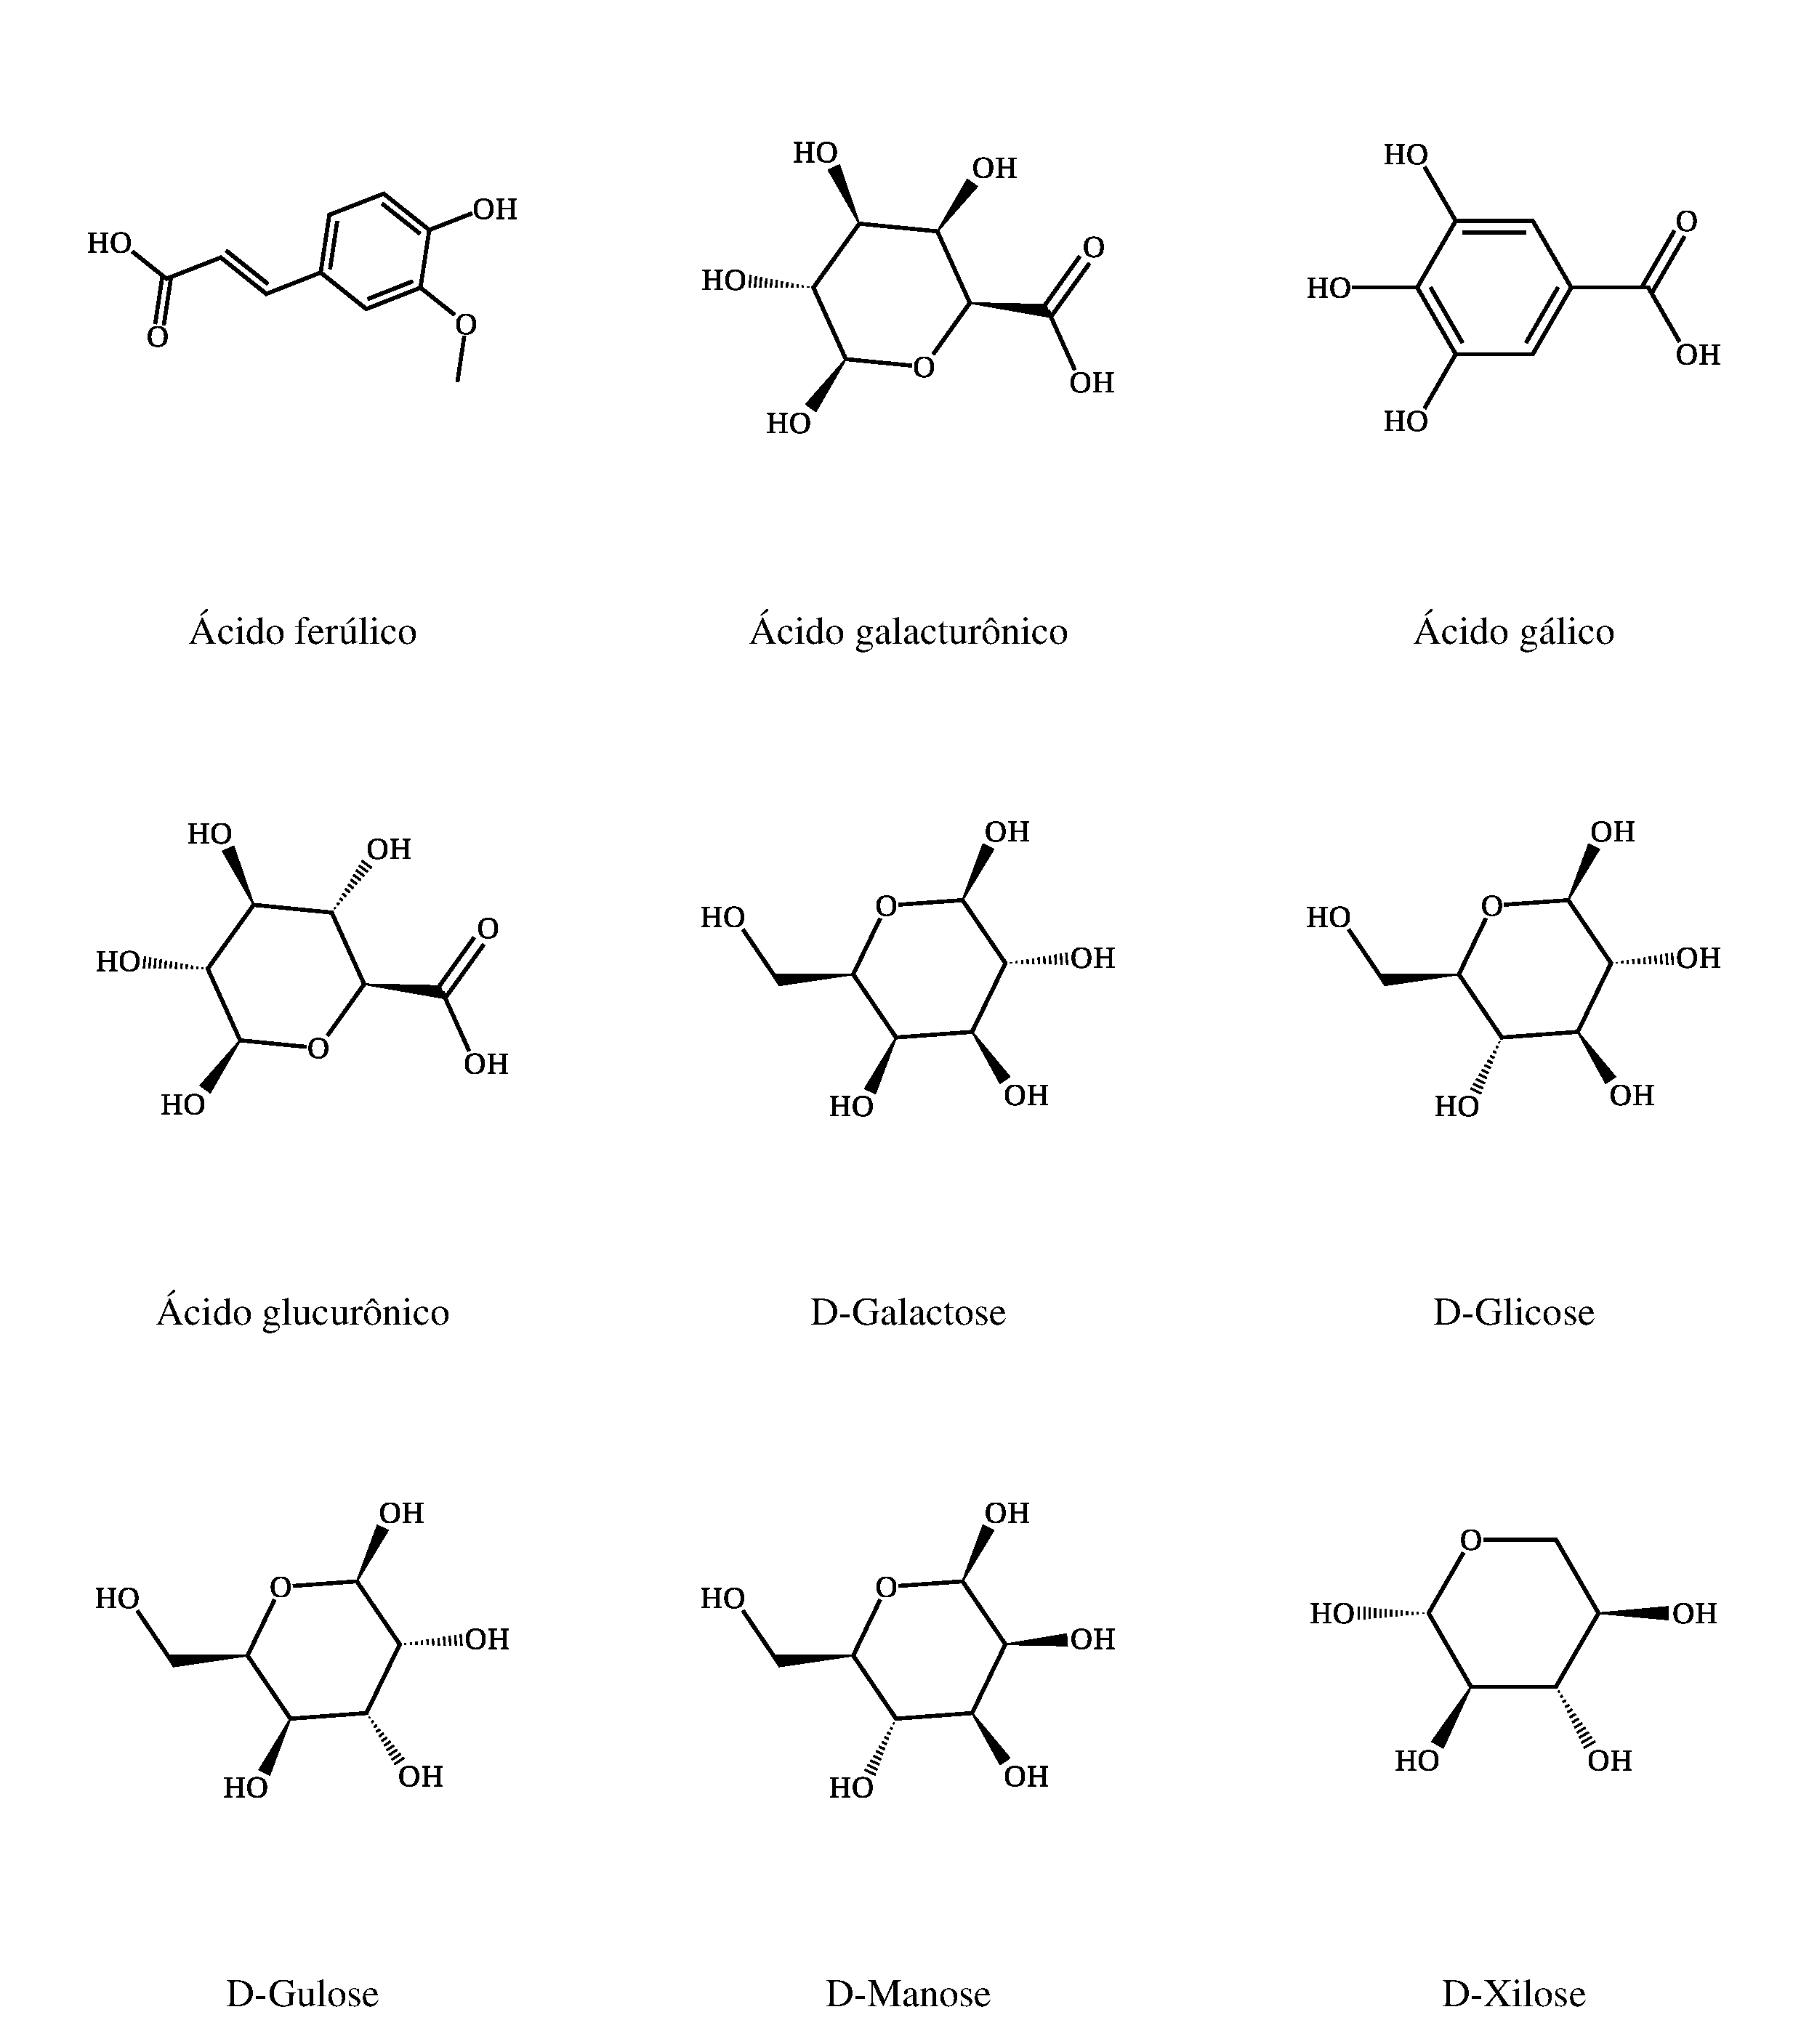
\includegraphics[width=\linewidth,height=18cm,keepaspectratio]{image/estruturas_ligantes_integracao/tetra_01.pdf}
\end{figure}

\clearpage
\begin{figure}[H]
\centering
\caption[Compostos para prospecção (2/2)]{Representações bidimensionais dos compostos selecionados para prospecção: painel 2 de 2, com os oito registros restantes. O asterisco identifica KDO e \(\alpha\)-Kdo, registros com o mesmo SMILES estereoquímico nos arquivos preparados.}
\label{fig:estruturas_tetra_02}
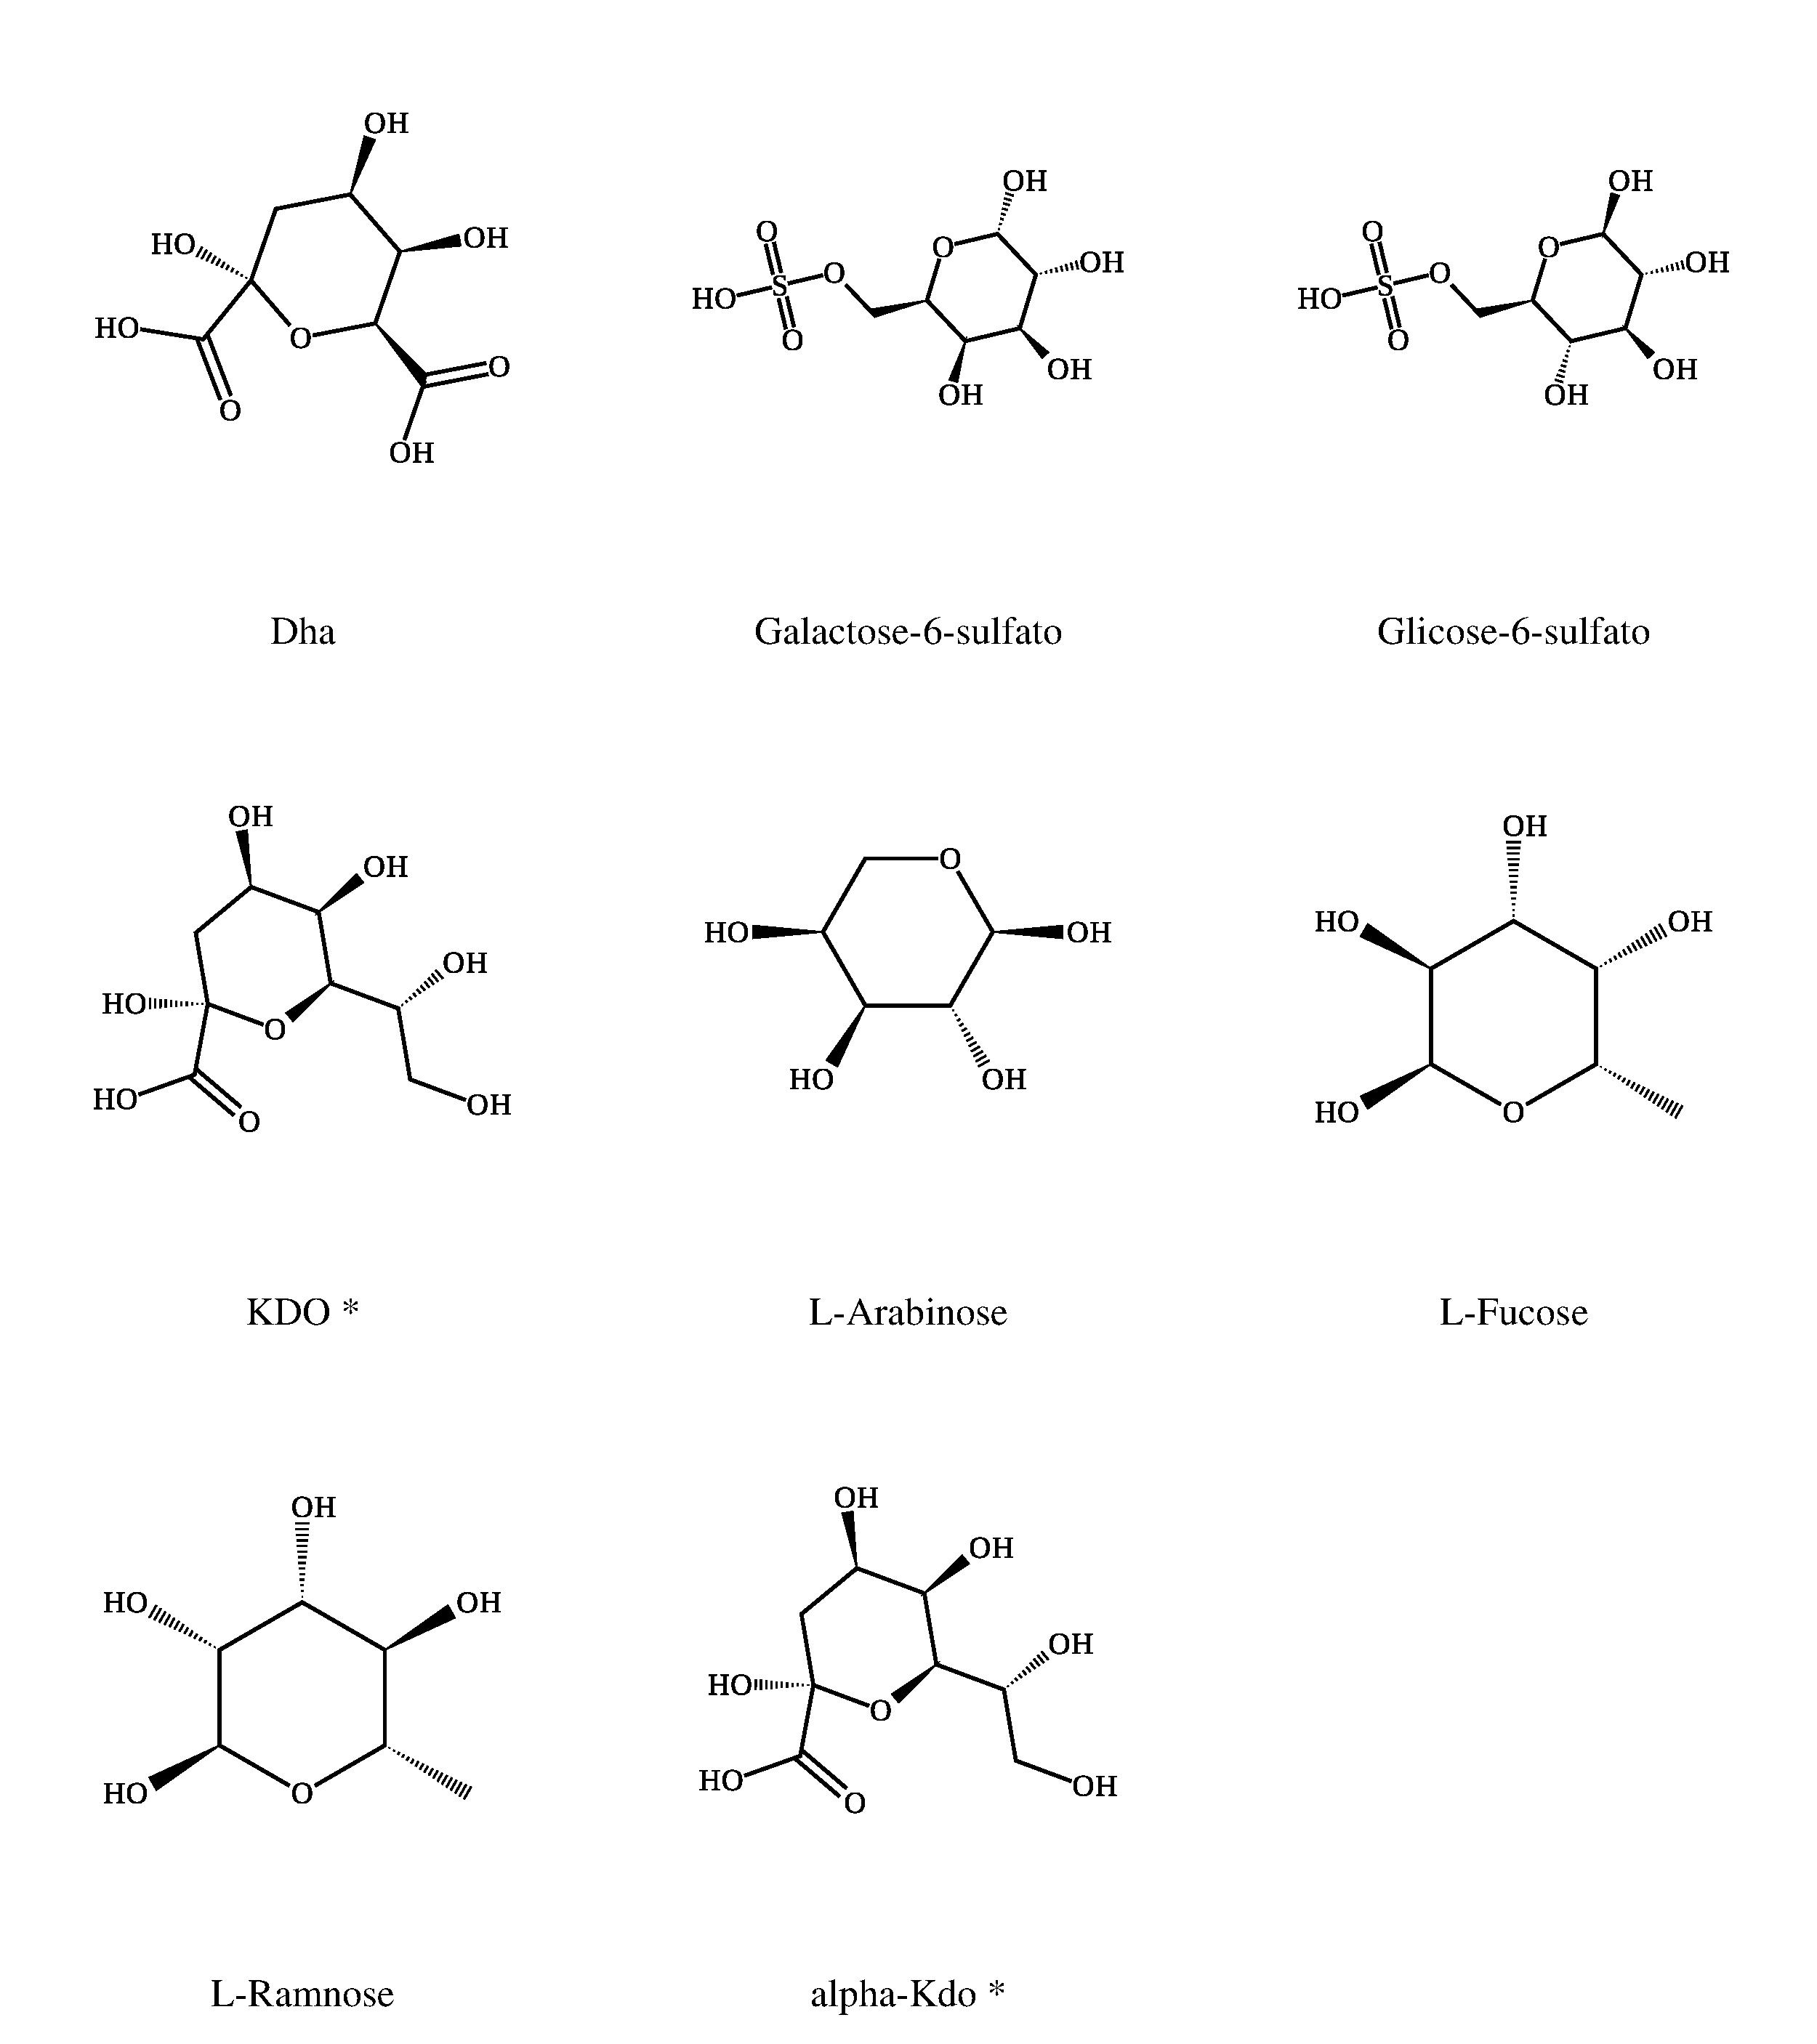
\includegraphics[width=\linewidth,height=17.4cm,keepaspectratio]{image/estruturas_ligantes_integracao/tetra_02.pdf}
\end{figure}

As 34 estruturas passaram pela sanitização do RDKit e pela conferência dos átomos pesados com o mapeamento \texttt{SMILES IDX}. KDO e \(\alpha\)-Kdo mantêm dois registros no inventário, mas possuem o mesmo SMILES estereoquímico; os desenhos não indicam moléculas distintas. As representações não determinam o estado de protonação em solução nem substituem uma identificação experimental. Nomes, SMILES, arquivos de origem, verificações e hashes SHA-256 constam no mapeamento suplementar, que preserva a rastreabilidade dos painéis.
